
%----------------------------------------------------------------------------------------%
% START LaTeX preamble

% define document type, font and paper size
\documentclass[11pt,a4paper]{article}

%----------------------------------------------------------------------------------------%
% IMPORT LaTeX packages

\usepackage{inputenc}
\usepackage[ngerman, english]{babel}
\usepackage{csquotes}
\usepackage{amsmath}
\usepackage{amssymb}
\usepackage{amsfonts}
\usepackage{graphicx}
\usepackage{wrapfig}
\usepackage[margin=1.25in]{geometry}
\usepackage{pdfpages}
\usepackage{listings}
\usepackage{setspace}
\usepackage{systeme}
\usepackage{mdframed}
\usepackage{mmacells}

\newcommand{\mathsym}[1]{{}}
\newcommand{\unicode}[1]{{}}

%----------------------------------------------------------------------------------------%
% IMPORT LaTeX packages to manange bibliography

% MLA, APA, or IEEE? - https://www.overleaf.com/learn/latex/Biblatex_citation_styles
\usepackage[style=apa, backend=biber]{biblatex}
\addbibresource{bibliography.bib}

%----------------------------------------------------------------------------------------%
% DEFINE header values

% define the cover page values
\title
{
    Mathematica Problem Sheet 01
}
\author
{    
    Antonio Osamu Katagiri Tanaka (A01212611) \\
    \\
    Instructor: Ph.D Daniel L{\' o}pez Aguayo
}
\date{\today}

%----------------------------------------------------------------------------------------%
% USER-DEFINED commands

% Keywords command
\providecommand{\keywords}[1]
{
    \\
    \\
    \small
    \textbf{\textit{Keywords:}} #1
}

%----------------------------------------------------------------------------------------%

\begin{document}
\setlength\parindent{0pt} % Set noindent for entire file

%----------------------------------------------------------------------------------------%
% CREATE the 1st page (cover page)

\maketitle

%----------------------------------------------------------------------------------------%
% DEFINE the abstract text & keywords

%\begin{abstract}
%    \emph
%    {
%        Lorem ipsum dolor sit amet, consectetur adipiscing elit, sed do eiusmod tempor incididunt ut labore et dolore magna aliqua. Ut enim ad minim veniam, quis nostrud exercitation ullamco laboris nisi ut aliquip ex ea commodo consequat. Duis aute irure dolor in reprehenderit in voluptate velit esse cillum dolore eu fugiat nulla pariatur. Excepteur sint occaecat cupidatat non proident, sunt in culpa qui officia deserunt mollit anim id est laborum.
%    }
%    \keywords{Lorem, ipsum, dolor, sit, amet}
%\end{abstract}
\clearpage

%----------------------------------------------------------------------------------------%
% CREATE a table of contents in a new page

%\tableofcontents
%\clearpage

%----------------------------------------------------------------------------------------%
% CREATE a list of figures and a list of tables in a new page

%\listoffigures
%\listoftables
%\clearpage

%----------------------------------------------------------------------------------------%
% DOCUMENT body starts here

%----------------------------------------------------------------------------------------%
%Append the HW's exercises
\includepdf[page=-]{MathematicaP1}

%----------------------------------------------------------------------------------------%
\section{Answer to Problem I}\label{sec:P01}

\begin{mmaCell}[moredefined={SQRmatrixSize, matrixAentries, matrixA, \
i, j}]{Input}
SQRmatrixSize=10;
matrixAentries =Range[1,SQRmatrixSize*SQRmatrixSize];
matrixAentries=ArrayReshape[matrixAentries,\{SQRmatrixSize,SQRmatrixSize\}];
matrixA=Table[matrixAentries[[i,j]],\{i,1,SQRmatrixSize\},\{j,1,SQRmatrixSize\}];
MatrixForm[matrixA]
\end{mmaCell}

\begin{mmaCell}[form=MatrixForm]{Output}

\end{mmaCell}

\begin{doublespace}
\noindent\(\left(
\begin{array}{cccccccccc}
 1 & 2 & 3 & 4 & 5 & 6 & 7 & 8 & 9 & 10 \\
 11 & 12 & 13 & 14 & 15 & 16 & 17 & 18 & 19 & 20 \\
 21 & 22 & 23 & 24 & 25 & 26 & 27 & 28 & 29 & 30 \\
 31 & 32 & 33 & 34 & 35 & 36 & 37 & 38 & 39 & 40 \\
 41 & 42 & 43 & 44 & 45 & 46 & 47 & 48 & 49 & 50 \\
 51 & 52 & 53 & 54 & 55 & 56 & 57 & 58 & 59 & 60 \\
 61 & 62 & 63 & 64 & 65 & 66 & 67 & 68 & 69 & 70 \\
 71 & 72 & 73 & 74 & 75 & 76 & 77 & 78 & 79 & 80 \\
 81 & 82 & 83 & 84 & 85 & 86 & 87 & 88 & 89 & 90 \\
 91 & 92 & 93 & 94 & 95 & 96 & 97 & 98 & 99 & 100 \\
\end{array}
\right)\)
\end{doublespace}

%----------------------------------------------------------------------------------------%
\section{Answer to Problem II}\label{sec:P02}

matrixA is singular, therefore Inverse[matrixA] does not exist.

\clearpage
%----------------------------------------------------------------------------------------%
\section{Answer to Problem III}\label{sec:P03}

\begin{mmaCell}[moredefined={SQRmatrixSize, matrixB}]{Input}
SQRmatrixSize=30;
matrixB=\mmaDef{\(\pmb{\pi}\)}*IdentityMatrix[SQRmatrixSize];
MatrixForm[matrixB]
\end{mmaCell}

\begin{mmaCell}[form=MatrixForm]{Output}

\end{mmaCell}

\begin{doublespace}
\noindent\(\left(
\begin{array}{cccccccccccccccccccccccccccccc}
 \pi  & 0 & 0 & 0 & 0 & 0 & 0 & 0 & 0 & 0 & 0 & 0 & 0 & 0 & 0 & 0 & 0 & 0 & 0 & 0 & 0 & 0 & 0 & 0 & 0 & 0 & 0 & 0 & 0 & 0 \\
 0 & \pi  & 0 & 0 & 0 & 0 & 0 & 0 & 0 & 0 & 0 & 0 & 0 & 0 & 0 & 0 & 0 & 0 & 0 & 0 & 0 & 0 & 0 & 0 & 0 & 0 & 0 & 0 & 0 & 0 \\
 0 & 0 & \pi  & 0 & 0 & 0 & 0 & 0 & 0 & 0 & 0 & 0 & 0 & 0 & 0 & 0 & 0 & 0 & 0 & 0 & 0 & 0 & 0 & 0 & 0 & 0 & 0 & 0 & 0 & 0 \\
 0 & 0 & 0 & \pi  & 0 & 0 & 0 & 0 & 0 & 0 & 0 & 0 & 0 & 0 & 0 & 0 & 0 & 0 & 0 & 0 & 0 & 0 & 0 & 0 & 0 & 0 & 0 & 0 & 0 & 0 \\
 0 & 0 & 0 & 0 & \pi  & 0 & 0 & 0 & 0 & 0 & 0 & 0 & 0 & 0 & 0 & 0 & 0 & 0 & 0 & 0 & 0 & 0 & 0 & 0 & 0 & 0 & 0 & 0 & 0 & 0 \\
 0 & 0 & 0 & 0 & 0 & \pi  & 0 & 0 & 0 & 0 & 0 & 0 & 0 & 0 & 0 & 0 & 0 & 0 & 0 & 0 & 0 & 0 & 0 & 0 & 0 & 0 & 0 & 0 & 0 & 0 \\
 0 & 0 & 0 & 0 & 0 & 0 & \pi  & 0 & 0 & 0 & 0 & 0 & 0 & 0 & 0 & 0 & 0 & 0 & 0 & 0 & 0 & 0 & 0 & 0 & 0 & 0 & 0 & 0 & 0 & 0 \\
 0 & 0 & 0 & 0 & 0 & 0 & 0 & \pi  & 0 & 0 & 0 & 0 & 0 & 0 & 0 & 0 & 0 & 0 & 0 & 0 & 0 & 0 & 0 & 0 & 0 & 0 & 0 & 0 & 0 & 0 \\
 0 & 0 & 0 & 0 & 0 & 0 & 0 & 0 & \pi  & 0 & 0 & 0 & 0 & 0 & 0 & 0 & 0 & 0 & 0 & 0 & 0 & 0 & 0 & 0 & 0 & 0 & 0 & 0 & 0 & 0 \\
 0 & 0 & 0 & 0 & 0 & 0 & 0 & 0 & 0 & \pi  & 0 & 0 & 0 & 0 & 0 & 0 & 0 & 0 & 0 & 0 & 0 & 0 & 0 & 0 & 0 & 0 & 0 & 0 & 0 & 0 \\
 0 & 0 & 0 & 0 & 0 & 0 & 0 & 0 & 0 & 0 & \pi  & 0 & 0 & 0 & 0 & 0 & 0 & 0 & 0 & 0 & 0 & 0 & 0 & 0 & 0 & 0 & 0 & 0 & 0 & 0 \\
 0 & 0 & 0 & 0 & 0 & 0 & 0 & 0 & 0 & 0 & 0 & \pi  & 0 & 0 & 0 & 0 & 0 & 0 & 0 & 0 & 0 & 0 & 0 & 0 & 0 & 0 & 0 & 0 & 0 & 0 \\
 0 & 0 & 0 & 0 & 0 & 0 & 0 & 0 & 0 & 0 & 0 & 0 & \pi  & 0 & 0 & 0 & 0 & 0 & 0 & 0 & 0 & 0 & 0 & 0 & 0 & 0 & 0 & 0 & 0 & 0 \\
 0 & 0 & 0 & 0 & 0 & 0 & 0 & 0 & 0 & 0 & 0 & 0 & 0 & \pi  & 0 & 0 & 0 & 0 & 0 & 0 & 0 & 0 & 0 & 0 & 0 & 0 & 0 & 0 & 0 & 0 \\
 0 & 0 & 0 & 0 & 0 & 0 & 0 & 0 & 0 & 0 & 0 & 0 & 0 & 0 & \pi  & 0 & 0 & 0 & 0 & 0 & 0 & 0 & 0 & 0 & 0 & 0 & 0 & 0 & 0 & 0 \\
 0 & 0 & 0 & 0 & 0 & 0 & 0 & 0 & 0 & 0 & 0 & 0 & 0 & 0 & 0 & \pi  & 0 & 0 & 0 & 0 & 0 & 0 & 0 & 0 & 0 & 0 & 0 & 0 & 0 & 0 \\
 0 & 0 & 0 & 0 & 0 & 0 & 0 & 0 & 0 & 0 & 0 & 0 & 0 & 0 & 0 & 0 & \pi  & 0 & 0 & 0 & 0 & 0 & 0 & 0 & 0 & 0 & 0 & 0 & 0 & 0 \\
 0 & 0 & 0 & 0 & 0 & 0 & 0 & 0 & 0 & 0 & 0 & 0 & 0 & 0 & 0 & 0 & 0 & \pi  & 0 & 0 & 0 & 0 & 0 & 0 & 0 & 0 & 0 & 0 & 0 & 0 \\
 0 & 0 & 0 & 0 & 0 & 0 & 0 & 0 & 0 & 0 & 0 & 0 & 0 & 0 & 0 & 0 & 0 & 0 & \pi  & 0 & 0 & 0 & 0 & 0 & 0 & 0 & 0 & 0 & 0 & 0 \\
 0 & 0 & 0 & 0 & 0 & 0 & 0 & 0 & 0 & 0 & 0 & 0 & 0 & 0 & 0 & 0 & 0 & 0 & 0 & \pi  & 0 & 0 & 0 & 0 & 0 & 0 & 0 & 0 & 0 & 0 \\
 0 & 0 & 0 & 0 & 0 & 0 & 0 & 0 & 0 & 0 & 0 & 0 & 0 & 0 & 0 & 0 & 0 & 0 & 0 & 0 & \pi  & 0 & 0 & 0 & 0 & 0 & 0 & 0 & 0 & 0 \\
 0 & 0 & 0 & 0 & 0 & 0 & 0 & 0 & 0 & 0 & 0 & 0 & 0 & 0 & 0 & 0 & 0 & 0 & 0 & 0 & 0 & \pi  & 0 & 0 & 0 & 0 & 0 & 0 & 0 & 0 \\
 0 & 0 & 0 & 0 & 0 & 0 & 0 & 0 & 0 & 0 & 0 & 0 & 0 & 0 & 0 & 0 & 0 & 0 & 0 & 0 & 0 & 0 & \pi  & 0 & 0 & 0 & 0 & 0 & 0 & 0 \\
 0 & 0 & 0 & 0 & 0 & 0 & 0 & 0 & 0 & 0 & 0 & 0 & 0 & 0 & 0 & 0 & 0 & 0 & 0 & 0 & 0 & 0 & 0 & \pi  & 0 & 0 & 0 & 0 & 0 & 0 \\
 0 & 0 & 0 & 0 & 0 & 0 & 0 & 0 & 0 & 0 & 0 & 0 & 0 & 0 & 0 & 0 & 0 & 0 & 0 & 0 & 0 & 0 & 0 & 0 & \pi  & 0 & 0 & 0 & 0 & 0 \\
 0 & 0 & 0 & 0 & 0 & 0 & 0 & 0 & 0 & 0 & 0 & 0 & 0 & 0 & 0 & 0 & 0 & 0 & 0 & 0 & 0 & 0 & 0 & 0 & 0 & \pi  & 0 & 0 & 0 & 0 \\
 0 & 0 & 0 & 0 & 0 & 0 & 0 & 0 & 0 & 0 & 0 & 0 & 0 & 0 & 0 & 0 & 0 & 0 & 0 & 0 & 0 & 0 & 0 & 0 & 0 & 0 & \pi  & 0 & 0 & 0 \\
 0 & 0 & 0 & 0 & 0 & 0 & 0 & 0 & 0 & 0 & 0 & 0 & 0 & 0 & 0 & 0 & 0 & 0 & 0 & 0 & 0 & 0 & 0 & 0 & 0 & 0 & 0 & \pi  & 0 & 0 \\
 0 & 0 & 0 & 0 & 0 & 0 & 0 & 0 & 0 & 0 & 0 & 0 & 0 & 0 & 0 & 0 & 0 & 0 & 0 & 0 & 0 & 0 & 0 & 0 & 0 & 0 & 0 & 0 & \pi  & 0 \\
 0 & 0 & 0 & 0 & 0 & 0 & 0 & 0 & 0 & 0 & 0 & 0 & 0 & 0 & 0 & 0 & 0 & 0 & 0 & 0 & 0 & 0 & 0 & 0 & 0 & 0 & 0 & 0 & 0 & \pi  \\
\end{array}
\right)\)
\end{doublespace}

3.a $\&$ 3.b\\
Yes, {``}A triangular matrix (upper, lower or diagonal) is invertible if and only if no element on its main diagonal is 0.{''}\\

{``}by hand{''} ...\\
Since, Inverse[A] equals diag($\frac{1}{a_1},\frac{1}{a_2},\ldots ,\frac{1}{a_n}$), Inverse[matrixB] is equal to $\frac{1}{\pi }$IdentityMatrix[30]\\

Verification with Mathematica is shown below ...

\begin{mmaCell}[moredefined={matrixB}]{Input}
Inverse[matrixB];
MatrixForm[%]
\end{mmaCell}

\begin{mmaCell}[form=MatrixForm]{Output}

\end{mmaCell}

\begin{doublespace}
\noindent\(\left(
\begin{array}{cccccccccccccccccccccccccccccc}
 \frac{1}{\pi } & 0 & 0 & 0 & 0 & 0 & 0 & 0 & 0 & 0 & 0 & 0 & 0 & 0 & 0 & 0 & 0 & 0 & 0 & 0 & 0 & 0 & 0 & 0 & 0 & 0 & 0 & 0 & 0 & 0 \\
 0 & \frac{1}{\pi } & 0 & 0 & 0 & 0 & 0 & 0 & 0 & 0 & 0 & 0 & 0 & 0 & 0 & 0 & 0 & 0 & 0 & 0 & 0 & 0 & 0 & 0 & 0 & 0 & 0 & 0 & 0 & 0 \\
 0 & 0 & \frac{1}{\pi } & 0 & 0 & 0 & 0 & 0 & 0 & 0 & 0 & 0 & 0 & 0 & 0 & 0 & 0 & 0 & 0 & 0 & 0 & 0 & 0 & 0 & 0 & 0 & 0 & 0 & 0 & 0 \\
 0 & 0 & 0 & \frac{1}{\pi } & 0 & 0 & 0 & 0 & 0 & 0 & 0 & 0 & 0 & 0 & 0 & 0 & 0 & 0 & 0 & 0 & 0 & 0 & 0 & 0 & 0 & 0 & 0 & 0 & 0 & 0 \\
 0 & 0 & 0 & 0 & \frac{1}{\pi } & 0 & 0 & 0 & 0 & 0 & 0 & 0 & 0 & 0 & 0 & 0 & 0 & 0 & 0 & 0 & 0 & 0 & 0 & 0 & 0 & 0 & 0 & 0 & 0 & 0 \\
 0 & 0 & 0 & 0 & 0 & \frac{1}{\pi } & 0 & 0 & 0 & 0 & 0 & 0 & 0 & 0 & 0 & 0 & 0 & 0 & 0 & 0 & 0 & 0 & 0 & 0 & 0 & 0 & 0 & 0 & 0 & 0 \\
 0 & 0 & 0 & 0 & 0 & 0 & \frac{1}{\pi } & 0 & 0 & 0 & 0 & 0 & 0 & 0 & 0 & 0 & 0 & 0 & 0 & 0 & 0 & 0 & 0 & 0 & 0 & 0 & 0 & 0 & 0 & 0 \\
 0 & 0 & 0 & 0 & 0 & 0 & 0 & \frac{1}{\pi } & 0 & 0 & 0 & 0 & 0 & 0 & 0 & 0 & 0 & 0 & 0 & 0 & 0 & 0 & 0 & 0 & 0 & 0 & 0 & 0 & 0 & 0 \\
 0 & 0 & 0 & 0 & 0 & 0 & 0 & 0 & \frac{1}{\pi } & 0 & 0 & 0 & 0 & 0 & 0 & 0 & 0 & 0 & 0 & 0 & 0 & 0 & 0 & 0 & 0 & 0 & 0 & 0 & 0 & 0 \\
 0 & 0 & 0 & 0 & 0 & 0 & 0 & 0 & 0 & \frac{1}{\pi } & 0 & 0 & 0 & 0 & 0 & 0 & 0 & 0 & 0 & 0 & 0 & 0 & 0 & 0 & 0 & 0 & 0 & 0 & 0 & 0 \\
 0 & 0 & 0 & 0 & 0 & 0 & 0 & 0 & 0 & 0 & \frac{1}{\pi } & 0 & 0 & 0 & 0 & 0 & 0 & 0 & 0 & 0 & 0 & 0 & 0 & 0 & 0 & 0 & 0 & 0 & 0 & 0 \\
 0 & 0 & 0 & 0 & 0 & 0 & 0 & 0 & 0 & 0 & 0 & \frac{1}{\pi } & 0 & 0 & 0 & 0 & 0 & 0 & 0 & 0 & 0 & 0 & 0 & 0 & 0 & 0 & 0 & 0 & 0 & 0 \\
 0 & 0 & 0 & 0 & 0 & 0 & 0 & 0 & 0 & 0 & 0 & 0 & \frac{1}{\pi } & 0 & 0 & 0 & 0 & 0 & 0 & 0 & 0 & 0 & 0 & 0 & 0 & 0 & 0 & 0 & 0 & 0 \\
 0 & 0 & 0 & 0 & 0 & 0 & 0 & 0 & 0 & 0 & 0 & 0 & 0 & \frac{1}{\pi } & 0 & 0 & 0 & 0 & 0 & 0 & 0 & 0 & 0 & 0 & 0 & 0 & 0 & 0 & 0 & 0 \\
 0 & 0 & 0 & 0 & 0 & 0 & 0 & 0 & 0 & 0 & 0 & 0 & 0 & 0 & \frac{1}{\pi } & 0 & 0 & 0 & 0 & 0 & 0 & 0 & 0 & 0 & 0 & 0 & 0 & 0 & 0 & 0 \\
 0 & 0 & 0 & 0 & 0 & 0 & 0 & 0 & 0 & 0 & 0 & 0 & 0 & 0 & 0 & \frac{1}{\pi } & 0 & 0 & 0 & 0 & 0 & 0 & 0 & 0 & 0 & 0 & 0 & 0 & 0 & 0 \\
 0 & 0 & 0 & 0 & 0 & 0 & 0 & 0 & 0 & 0 & 0 & 0 & 0 & 0 & 0 & 0 & \frac{1}{\pi } & 0 & 0 & 0 & 0 & 0 & 0 & 0 & 0 & 0 & 0 & 0 & 0 & 0 \\
 0 & 0 & 0 & 0 & 0 & 0 & 0 & 0 & 0 & 0 & 0 & 0 & 0 & 0 & 0 & 0 & 0 & \frac{1}{\pi } & 0 & 0 & 0 & 0 & 0 & 0 & 0 & 0 & 0 & 0 & 0 & 0 \\
 0 & 0 & 0 & 0 & 0 & 0 & 0 & 0 & 0 & 0 & 0 & 0 & 0 & 0 & 0 & 0 & 0 & 0 & \frac{1}{\pi } & 0 & 0 & 0 & 0 & 0 & 0 & 0 & 0 & 0 & 0 & 0 \\
 0 & 0 & 0 & 0 & 0 & 0 & 0 & 0 & 0 & 0 & 0 & 0 & 0 & 0 & 0 & 0 & 0 & 0 & 0 & \frac{1}{\pi } & 0 & 0 & 0 & 0 & 0 & 0 & 0 & 0 & 0 & 0 \\
 0 & 0 & 0 & 0 & 0 & 0 & 0 & 0 & 0 & 0 & 0 & 0 & 0 & 0 & 0 & 0 & 0 & 0 & 0 & 0 & \frac{1}{\pi } & 0 & 0 & 0 & 0 & 0 & 0 & 0 & 0 & 0 \\
 0 & 0 & 0 & 0 & 0 & 0 & 0 & 0 & 0 & 0 & 0 & 0 & 0 & 0 & 0 & 0 & 0 & 0 & 0 & 0 & 0 & \frac{1}{\pi } & 0 & 0 & 0 & 0 & 0 & 0 & 0 & 0 \\
 0 & 0 & 0 & 0 & 0 & 0 & 0 & 0 & 0 & 0 & 0 & 0 & 0 & 0 & 0 & 0 & 0 & 0 & 0 & 0 & 0 & 0 & \frac{1}{\pi } & 0 & 0 & 0 & 0 & 0 & 0 & 0 \\
 0 & 0 & 0 & 0 & 0 & 0 & 0 & 0 & 0 & 0 & 0 & 0 & 0 & 0 & 0 & 0 & 0 & 0 & 0 & 0 & 0 & 0 & 0 & \frac{1}{\pi } & 0 & 0 & 0 & 0 & 0 & 0 \\
 0 & 0 & 0 & 0 & 0 & 0 & 0 & 0 & 0 & 0 & 0 & 0 & 0 & 0 & 0 & 0 & 0 & 0 & 0 & 0 & 0 & 0 & 0 & 0 & \frac{1}{\pi } & 0 & 0 & 0 & 0 & 0 \\
 0 & 0 & 0 & 0 & 0 & 0 & 0 & 0 & 0 & 0 & 0 & 0 & 0 & 0 & 0 & 0 & 0 & 0 & 0 & 0 & 0 & 0 & 0 & 0 & 0 & \frac{1}{\pi } & 0 & 0 & 0 & 0 \\
 0 & 0 & 0 & 0 & 0 & 0 & 0 & 0 & 0 & 0 & 0 & 0 & 0 & 0 & 0 & 0 & 0 & 0 & 0 & 0 & 0 & 0 & 0 & 0 & 0 & 0 & \frac{1}{\pi } & 0 & 0 & 0 \\
 0 & 0 & 0 & 0 & 0 & 0 & 0 & 0 & 0 & 0 & 0 & 0 & 0 & 0 & 0 & 0 & 0 & 0 & 0 & 0 & 0 & 0 & 0 & 0 & 0 & 0 & 0 & \frac{1}{\pi } & 0 & 0 \\
 0 & 0 & 0 & 0 & 0 & 0 & 0 & 0 & 0 & 0 & 0 & 0 & 0 & 0 & 0 & 0 & 0 & 0 & 0 & 0 & 0 & 0 & 0 & 0 & 0 & 0 & 0 & 0 & \frac{1}{\pi } & 0 \\
 0 & 0 & 0 & 0 & 0 & 0 & 0 & 0 & 0 & 0 & 0 & 0 & 0 & 0 & 0 & 0 & 0 & 0 & 0 & 0 & 0 & 0 & 0 & 0 & 0 & 0 & 0 & 0 & 0 & \frac{1}{\pi } \\
\end{array}
\right)\)
\end{doublespace}

3.c

\begin{mmaCell}[moredefined={matrixB}]{Input}
MatrixRank[matrixB]
\end{mmaCell}

\begin{mmaCell}{Output}
30
\end{mmaCell}

\clearpage
%----------------------------------------------------------------------------------------%
\section{Answer to Problem IV}\label{sec:P04}

\begin{mmaCell}[moredefined={SQRmatrixSize, matrixC, i, j, rows, cols}]{Input}
SQRmatrixSize=16;
matrixC=Table[0,\{i,1,SQRmatrixSize\},\{j,1,\
SQRmatrixSize\}];
rows=Dimensions[matrixC][[1]];
cols=Dimensions[matrixC][[2]];
For[i=1,i\(\pmb{\leq}\)rows,i++,
  For[j=1,j\(\pmb{\leq}\)cols,j++,
    If[i==j,
      matrixC[[i,j]]=(\mmaDef{\(\pmb{\pi}\)}+i)-1,
      matrixC[[i,j]]=0];
  ];
];
MatrixForm[matrixC]
\end{mmaCell}

\begin{mmaCell}[form=MatrixForm]{Output}

\end{mmaCell}

\begin{doublespace}
\noindent\(\left(
\begin{array}{cccccccccccccccc}
 \pi  & 0 & 0 & 0 & 0 & 0 & 0 & 0 & 0 & 0 & 0 & 0 & 0 & 0 & 0 & 0 \\
 0 & 1+\pi  & 0 & 0 & 0 & 0 & 0 & 0 & 0 & 0 & 0 & 0 & 0 & 0 & 0 & 0 \\
 0 & 0 & 2+\pi  & 0 & 0 & 0 & 0 & 0 & 0 & 0 & 0 & 0 & 0 & 0 & 0 & 0 \\
 0 & 0 & 0 & 3+\pi  & 0 & 0 & 0 & 0 & 0 & 0 & 0 & 0 & 0 & 0 & 0 & 0 \\
 0 & 0 & 0 & 0 & 4+\pi  & 0 & 0 & 0 & 0 & 0 & 0 & 0 & 0 & 0 & 0 & 0 \\
 0 & 0 & 0 & 0 & 0 & 5+\pi  & 0 & 0 & 0 & 0 & 0 & 0 & 0 & 0 & 0 & 0 \\
 0 & 0 & 0 & 0 & 0 & 0 & 6+\pi  & 0 & 0 & 0 & 0 & 0 & 0 & 0 & 0 & 0 \\
 0 & 0 & 0 & 0 & 0 & 0 & 0 & 7+\pi  & 0 & 0 & 0 & 0 & 0 & 0 & 0 & 0 \\
 0 & 0 & 0 & 0 & 0 & 0 & 0 & 0 & 8+\pi  & 0 & 0 & 0 & 0 & 0 & 0 & 0 \\
 0 & 0 & 0 & 0 & 0 & 0 & 0 & 0 & 0 & 9+\pi  & 0 & 0 & 0 & 0 & 0 & 0 \\
 0 & 0 & 0 & 0 & 0 & 0 & 0 & 0 & 0 & 0 & 10+\pi  & 0 & 0 & 0 & 0 & 0 \\
 0 & 0 & 0 & 0 & 0 & 0 & 0 & 0 & 0 & 0 & 0 & 11+\pi  & 0 & 0 & 0 & 0 \\
 0 & 0 & 0 & 0 & 0 & 0 & 0 & 0 & 0 & 0 & 0 & 0 & 12+\pi  & 0 & 0 & 0 \\
 0 & 0 & 0 & 0 & 0 & 0 & 0 & 0 & 0 & 0 & 0 & 0 & 0 & 13+\pi  & 0 & 0 \\
 0 & 0 & 0 & 0 & 0 & 0 & 0 & 0 & 0 & 0 & 0 & 0 & 0 & 0 & 14+\pi  & 0 \\
 0 & 0 & 0 & 0 & 0 & 0 & 0 & 0 & 0 & 0 & 0 & 0 & 0 & 0 & 0 & 15+\pi  \\
\end{array}
\right)\)
\end{doublespace}

\clearpage

4.a $\&$ 4.b\\
Yes, {``}A triangular matrix (upper, lower or diagonal) is invertible if and only if no element on its main diagonal is 0.{''}\\
\\
{``}by hand{''} ...\\
Since, Inverse[A] equals diag($\frac{1}{a_1},\frac{1}{a_2},\ldots ,\frac{1}{a_n}$), Inverse[matrixB] is equal to $\frac{1}{(\pi +i)-1}$IdentityMatrix[16]\\
\\
Verification with Mathematica is shown below ...

\begin{mmaCell}[moredefined={matrixC}]{Input}
Inverse[matrixC];
MatrixForm[%]
\end{mmaCell}

\begin{mmaCell}{Output}

\end{mmaCell}

\begin{doublespace}
\noindent\(\left(
\begin{array}{cccccccccccccccc}
 \frac{1}{\pi } & 0 & 0 & 0 & 0 & 0 & 0 & 0 & 0 & 0 & 0 & 0 & 0 & 0 & 0 & 0 \\
 0 & \frac{1}{1+\pi } & 0 & 0 & 0 & 0 & 0 & 0 & 0 & 0 & 0 & 0 & 0 & 0 & 0 & 0 \\
 0 & 0 & \frac{1}{2+\pi } & 0 & 0 & 0 & 0 & 0 & 0 & 0 & 0 & 0 & 0 & 0 & 0 & 0 \\
 0 & 0 & 0 & \frac{1}{3+\pi } & 0 & 0 & 0 & 0 & 0 & 0 & 0 & 0 & 0 & 0 & 0 & 0 \\
 0 & 0 & 0 & 0 & \frac{1}{4+\pi } & 0 & 0 & 0 & 0 & 0 & 0 & 0 & 0 & 0 & 0 & 0 \\
 0 & 0 & 0 & 0 & 0 & \frac{1}{5+\pi } & 0 & 0 & 0 & 0 & 0 & 0 & 0 & 0 & 0 & 0 \\
 0 & 0 & 0 & 0 & 0 & 0 & \frac{1}{6+\pi } & 0 & 0 & 0 & 0 & 0 & 0 & 0 & 0 & 0 \\
 0 & 0 & 0 & 0 & 0 & 0 & 0 & \frac{1}{7+\pi } & 0 & 0 & 0 & 0 & 0 & 0 & 0 & 0 \\
 0 & 0 & 0 & 0 & 0 & 0 & 0 & 0 & \frac{1}{8+\pi } & 0 & 0 & 0 & 0 & 0 & 0 & 0 \\
 0 & 0 & 0 & 0 & 0 & 0 & 0 & 0 & 0 & \frac{1}{9+\pi } & 0 & 0 & 0 & 0 & 0 & 0 \\
 0 & 0 & 0 & 0 & 0 & 0 & 0 & 0 & 0 & 0 & \frac{1}{10+\pi } & 0 & 0 & 0 & 0 & 0 \\
 0 & 0 & 0 & 0 & 0 & 0 & 0 & 0 & 0 & 0 & 0 & \frac{1}{11+\pi } & 0 & 0 & 0 & 0 \\
 0 & 0 & 0 & 0 & 0 & 0 & 0 & 0 & 0 & 0 & 0 & 0 & \frac{1}{12+\pi } & 0 & 0 & 0 \\
 0 & 0 & 0 & 0 & 0 & 0 & 0 & 0 & 0 & 0 & 0 & 0 & 0 & \frac{1}{13+\pi } & 0 & 0 \\
 0 & 0 & 0 & 0 & 0 & 0 & 0 & 0 & 0 & 0 & 0 & 0 & 0 & 0 & \frac{1}{14+\pi } & 0 \\
 0 & 0 & 0 & 0 & 0 & 0 & 0 & 0 & 0 & 0 & 0 & 0 & 0 & 0 & 0 & \frac{1}{15+\pi } \\
\end{array}
\right)\)
\end{doublespace}

\clearpage

4.c\\
Multiplying matrixC times the inverse of matrixC. However, since we know that Inverse[matrixC] exists, the reduced echelon form is the identity matrix
(of size 16x16).

\begin{mmaCell}[moredefined={matrixC}]{Input}
MatrixRank[matrixC];
RowReduce[matrixC];
MatrixForm[%]
\end{mmaCell}

\begin{mmaCell}[form=MatrixForm]{Output}

\end{mmaCell}

\begin{doublespace}
\noindent\(\left(
\begin{array}{cccccccccccccccc}
 1 & 0 & 0 & 0 & 0 & 0 & 0 & 0 & 0 & 0 & 0 & 0 & 0 & 0 & 0 & 0 \\
 0 & 1 & 0 & 0 & 0 & 0 & 0 & 0 & 0 & 0 & 0 & 0 & 0 & 0 & 0 & 0 \\
 0 & 0 & 1 & 0 & 0 & 0 & 0 & 0 & 0 & 0 & 0 & 0 & 0 & 0 & 0 & 0 \\
 0 & 0 & 0 & 1 & 0 & 0 & 0 & 0 & 0 & 0 & 0 & 0 & 0 & 0 & 0 & 0 \\
 0 & 0 & 0 & 0 & 1 & 0 & 0 & 0 & 0 & 0 & 0 & 0 & 0 & 0 & 0 & 0 \\
 0 & 0 & 0 & 0 & 0 & 1 & 0 & 0 & 0 & 0 & 0 & 0 & 0 & 0 & 0 & 0 \\
 0 & 0 & 0 & 0 & 0 & 0 & 1 & 0 & 0 & 0 & 0 & 0 & 0 & 0 & 0 & 0 \\
 0 & 0 & 0 & 0 & 0 & 0 & 0 & 1 & 0 & 0 & 0 & 0 & 0 & 0 & 0 & 0 \\
 0 & 0 & 0 & 0 & 0 & 0 & 0 & 0 & 1 & 0 & 0 & 0 & 0 & 0 & 0 & 0 \\
 0 & 0 & 0 & 0 & 0 & 0 & 0 & 0 & 0 & 1 & 0 & 0 & 0 & 0 & 0 & 0 \\
 0 & 0 & 0 & 0 & 0 & 0 & 0 & 0 & 0 & 0 & 1 & 0 & 0 & 0 & 0 & 0 \\
 0 & 0 & 0 & 0 & 0 & 0 & 0 & 0 & 0 & 0 & 0 & 1 & 0 & 0 & 0 & 0 \\
 0 & 0 & 0 & 0 & 0 & 0 & 0 & 0 & 0 & 0 & 0 & 0 & 1 & 0 & 0 & 0 \\
 0 & 0 & 0 & 0 & 0 & 0 & 0 & 0 & 0 & 0 & 0 & 0 & 0 & 1 & 0 & 0 \\
 0 & 0 & 0 & 0 & 0 & 0 & 0 & 0 & 0 & 0 & 0 & 0 & 0 & 0 & 1 & 0 \\
 0 & 0 & 0 & 0 & 0 & 0 & 0 & 0 & 0 & 0 & 0 & 0 & 0 & 0 & 0 & 1 \\
\end{array}
\right)\)
\end{doublespace}

\clearpage
%----------------------------------------------------------------------------------------%
\section{Answer to Problem V}\label{sec:P05}

5.a\\
\begin{mmaCell}[moredefined={matrixD}]{Input}
matrixD=\{\{a,b\},\{c,d\}\};
Inverse[matrixD];
MatrixForm[%]
\end{mmaCell}

\begin{mmaCell}[form=MatrixForm]{Output}

\end{mmaCell}

\begin{doublespace}
\noindent\(\left(
\begin{array}{cc}
 \frac{d}{-b c+a d} & -\frac{b}{-b c+a d} \\
 -\frac{c}{-b c+a d} & \frac{a}{-b c+a d} \\
\end{array}
\right)\)
\end{doublespace}

5.b\\
When { }a = 2; d = 2; b = 1; c = 4, Inverse[matrixD] does not exist. Mathematica outputs the following error:\\
$\cdots $ Inverse: Matrix $\{\{$2,1$\}$,$\{$4,2$\}\}$ is singular

\clearpage
%----------------------------------------------------------------------------------------%
\section{Answer to Problem VI}\label{sec:P06}

6.a\\
\begin{mmaCell}[morefunctionlocal={x, y}]{Input}
Solve[\{
  x-y==3,
  x*\mmaDef{\(\pmb{\pi}\)}-y*\mmaDef{\(\pmb{\pi}\)}==3*\mmaDef{\(\pmb{\pi}\)}
\},\{x,y\}]
\end{mmaCell}

Solve: Equations may not give solutions for all "solve" variables.

\begin{mmaCell}{Output}
\{\{y\(\to\)-3+x\}\}
\end{mmaCell}

6.b\\
\begin{mmaCell}[moredefined={contourLimits},morefunctionlocal={x}]{Input}
contourLimits=2.5;
(*
ContourPlot[\{
  x-y==3,
  x*\(\pmb{\pi}\)-y*\(\pmb{\pi}\)==3*\(\pmb{\pi}\)
\},\{x,0.5,1.0\},\{y,-2.0,-2.5\},ContourStyle\(\pmb{\to}\)\{Blue,Orange\}]
*)
Show[\{
  Plot[x-3,\{x,-contourLimits,contourLimits\},PlotStyle\(\pmb{\to}\)Blue],
  Plot[x-3,\{x,-contourLimits,contourLimits\},PlotStyle\(\pmb{\to}\)Green]
\},PlotRange\(\pmb{\to}\)All,AxesOrigin \(\pmb{\to}\)\{0,0\}]
\end{mmaCell}

\includegraphics{MathematicaP1_gr1.eps}

6.c\\
The system has infinitely many solutions.

\clearpage
6.d\\
\begin{mmaCell}[addtoindex=1,moredefined={matrixA, matrixB, getNumOfSolutions},morepattern={varA_, varB_, varA, varB},morelocal={vA, vB, vAB, Arank, ABrank, n}]{Input}
matrixA=\{\{1,-1\},\{\mmaDef{\(\pmb{\pi}\)},-\mmaDef{\(\pmb{\pi}\)}\}\};
matrixB=\{\{3\},\{3*\mmaDef{\(\pmb{\pi}\)}\}\};

(* rows=m=i *) (* cols=n=j *)
getNumOfSolutions[varA_,varB_]:=Module[\{vA=varA,vB=varB,vAB,Arank,ABrank,n\},
  vAB=ArrayFlatten[\{\{vA,vB\}\}];
  Arank=MatrixRank[vA];
  ABrank=MatrixRank[vAB];
  n=Dimensions[vA][[2]];
  If[Arank<ABrank,
    Print["The system has no solution"];,
    If[Arank==ABrank&&Arank<n&&ABrank<n,
      Print["The system has infinitely many solutions"];,
      If[Arank==ABrank&&Arank==n,
        Print["The system has a unique solution"];,
        Print["[ERROR] The system has ? solution(s)\textbackslash{}n
          Beware, if the system is homogeneous (varB is a zero vector
          and n>m (more variables than equations), then the system has
          infinitely many solutions)"];
      ];
    ];
  ];
];

getNumOfSolutions[matrixA,matrixB]
\end{mmaCell}

\begin{mmaCell}{Print}
The system has infinitely many solutions
\end{mmaCell}

\clearpage
%----------------------------------------------------------------------------------------%
\section{Answer to Problem VII}\label{sec:P07}

7.a\\
\begin{mmaCell}[addtoindex=3,moredefined={contourLimits},morefunctionlocal={x, y}]{Input}
contourLimits=5;
(*
ContourPlot3D[\{
  x+y+z==10,
  \mmaFrac{2}{3}*x+\mmaFrac{2}{3}*y+\mmaFrac{2}{3}*z==11,
  \mmaFrac{5}{9}*x+\mmaFrac{5}{9}*y+\mmaFrac{5}{9}*z==12
\},
\{x,-contourLimits,contourLimits\},
\{y,-contourLimits,contourLimits\},
\{z,-contourLimits,contourLimits\},Axes\(\pmb{\to}\)True,PlotLegends\(\pmb{\to}\)"Expressions"]
*)
Show[\{
  Plot3D[10-x-y,
    \{x,-contourLimits,contourLimits\},\{y,-contourLimits,contourLimits\},
    PlotStyle\(\pmb{\to}\)Blue],
  Plot3D[\mmaFrac{1}{2} (33-2 x-2 y),
    \{x,-contourLimits,contourLimits\},\{y,-contourLimits,contourLimits\},
    PlotStyle\(\pmb{\to}\)Orange],
  Plot3D[\mmaFrac{1}{5} (108-5 x-5 y),
    \{x,-contourLimits,contourLimits\},\{y,-contourLimits,contourLimits\},
    PlotStyle\(\pmb{\to}\)Green]
\},PlotRange\(\pmb{\to}\)All,AxesOrigin \(\pmb{\to}\)\{0,0\}]
\end{mmaCell}

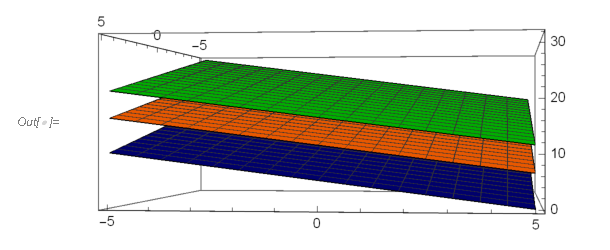
\includegraphics{MathematicaP1_gr2.eps}

7.b\\
7.b.1 \pmb{ normal vector:} A non-zero vector that is perpendicular to the plane is called a normal vector to the plane, as shown in Figure \ref{img:01}. \parencite{Kuttler}

\begin{figure}[!htbp]
\centering
\includegraphics[width=0.60\textwidth]{normalv.png}
\caption{Given a non-zero vector n in R3 and a point P, there exists a unique plane that contains P and has n as a normal vector. \parencite{Kuttler} Q is an arbitrary point on the plane, and is irrelevant for this exercise. \label{img:01}}
\end{figure}

7.b.2 The system is inconsistent because the three normal vectors point to the same direction.\\

7.c\\
\begin{mmaCell}[addtoindex=1,morefunctionlocal={x, y, z}]{Input}
Solve[\{
x+y+z==10,
\mmaFrac{2}{3}*x+\mmaFrac{2}{3}*y+\mmaFrac{2}{3}*z==11,
\mmaFrac{5}{9}*x+\mmaFrac{5}{9}*y+\mmaFrac{5}{9}*z==12
\},\{x,y,z\}]
\end{mmaCell}

\begin{mmaCell}{Output}
\{\}
\end{mmaCell}

7.d $\&$ 7.e\\
The reduced row echelon of A will be \(\left(
\begin{array}{ccc}
 1 & 1 & 1 \\
 0 & 0 & 0 \\
 0 & 0 & 0 \\
\end{array}
\right)\), since all the entries are the same within each row. MatrixRank[A]=1\\
\\
Verification with Mathematica is shown below ...

\begin{doublespace}
\noindent\(\pmb{\text{matrixA}=\left(
\begin{array}{ccc}
 1 & 1 & 1 \\
 \frac{2}{3} & \frac{2}{3} & \frac{2}{3} \\
 \frac{5}{9} & \frac{5}{9} & \frac{5}{9} \\
\end{array}
\right);}\\
\pmb{\text{matrixB}=\left(
\begin{array}{c}
 10 \\
 11 \\
 12 \\
\end{array}
\right);}\\
\pmb{\text{matrixAB}=\text{ArrayFlatten}[\{\{\text{matrixA},\text{matrixB}\}\}];}\\
\pmb{\text{RowReduce}[\text{matrixA}]}\\
\pmb{\text{MatrixForm}[\%]}\\
\pmb{\text{MatrixRank}[\text{matrixA}]}\)
\end{doublespace}

\begin{doublespace}
\noindent\(\{\{1,1,1\},\{0,0,0\},\{0,0,0\}\}\)
\end{doublespace}

\begin{doublespace}
\noindent\(\left(
\begin{array}{ccc}
 1 & 1 & 1 \\
 0 & 0 & 0 \\
 0 & 0 & 0 \\
\end{array}
\right)\)
\end{doublespace}

\begin{doublespace}
\noindent\(1\)
\end{doublespace}

7.f\\
\begin{doublespace}
\noindent\(\pmb{\text{RowReduce}[\text{matrixAB}];}\\
\pmb{\text{MatrixForm}[\%]}\\
\pmb{\text{MatrixRank}[\text{matrixAB}]}\)
\end{doublespace}

\begin{doublespace}
\noindent\(\left(
\begin{array}{cccc}
 1 & 1 & 1 & 0 \\
 0 & 0 & 0 & 1 \\
 0 & 0 & 0 & 0 \\
\end{array}
\right)\)
\end{doublespace}

\begin{doublespace}
\noindent\(2\)
\end{doublespace}


7.g\\
\begin{doublespace}
\noindent\(\pmb{\text{getNumOfSolutions}[\text{matrixA},\text{matrixB}]}\)
\end{doublespace}

\noindent\(\text{The system has no solution}\)

\clearpage
%----------------------------------------------------------------------------------------%
\section{Mathematica LaTeX tests}\label{sec:P08}



\clearpage
%----------------------------------------------------------------------------------------%
% PRINT bibliography/references in a new page

%\clearpage
\printbibliography

%----------------------------------------------------------------------------------------%

\end{document}

%----------------------------------------------------------------------------------------%
